\documentclass{article}
\usepackage{graphicx} % new way of doing eps files
\usepackage{listings} % nice code layout
\usepackage[usenames]{color} % color
\definecolor{listinggray}{gray}{0.9}
\definecolor{graphgray}{gray}{0.7}
\definecolor{ans}{rgb}{1,0,0}
\definecolor{blue}{rgb}{0,0,1}
% \Verilog{title}{label}{file}
\newcommand{\Verilog}[3]{
  \lstset{language=Verilog}
  \lstset{backgroundcolor=\color{listinggray},rulecolor=\color{blue}}
  \lstset{linewidth=\textwidth}
  \lstset{commentstyle=\textit, stringstyle=\upshape,showspaces=false}
  \lstset{frame=tb}
  \lstinputlisting[caption={#1},label={#2}]{#3}
}


\author{your names}
\title{Lab title}

\begin{document}
\maketitle

\section{Introduction}
Write one paragraph to explain the big picture of the lab.

\section{Interface}
This section should identify the inputs and outputs of each stage.  To do this, rather than explaining them in paragraph form, please take the datapath diagram in Figure ~\ref{fig:datapath} and add your signal names to the diagram.  This will give you a graphical representation of your system that can be quickly evaluated to determine the meaning of each signal.  For any additional signals that appear on your simulation results, put the signals in a table with a short description of that signal.

\begin{figure}
	\caption{Full Non-Pipelined Datapath}\label{fig:datapath}
	\begin{center}
		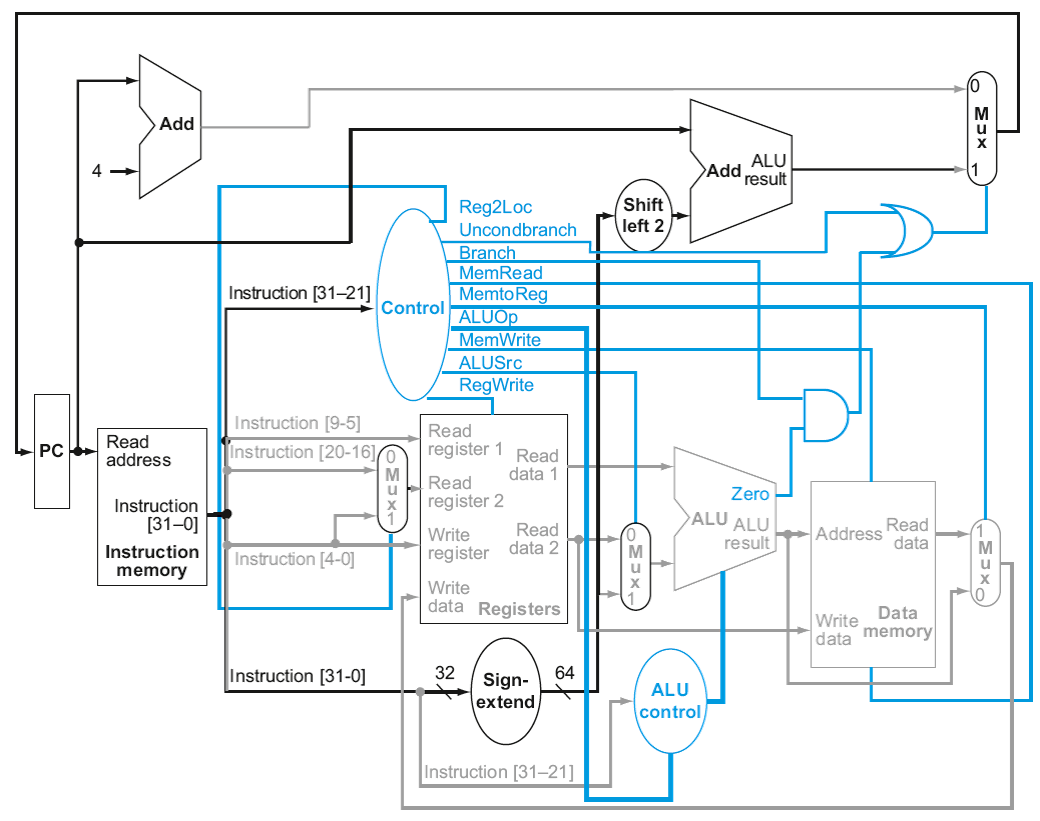
\includegraphics[width=\textwidth]{../images/non_pipelined_datapath.png}
	\end{center}
\end{figure}

\section{Design}
Most of the design for the datapath is pre-determined by Figure ~\ref{fig:datapath}.  The item that is not pre-determined is the timing.  For this Design section, you do not need to add any text.  Please just include a timing diagram that shows the timing between each stage.  See Figure ~\ref{fig:timing_diagram_example} for an example of a simple timing diagram.

\begin{figure}
	\caption{Timing Diagram Example}\label{fig:timing_diagram_example}
	\begin{center}
		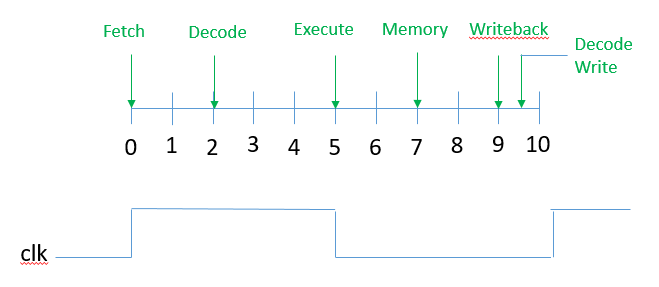
\includegraphics[width=\textwidth]{../images/timing_diagram_example.png}
	\end{center}
\end{figure}

\section{Implementation}
In this section, please just include your datapath.v code.  No text is necessary for this section.

\section{Test}
For this section, no text is necessary.  Please include:
\begin{enumerate}
	\item Assembly code for the "Division Problem" C code that I gave you
	\item Instruction Data File for the Division Problem
	\item Register Data File for the Division Problem
	\item Memory Data File for the Division Problem
	\item Simulation Results for the Division Problem
\end{enumerate}

\section{Conclusions}
Overview the main points you want to stick in peoples minds and answer key questions you want to stick in peoples minds.  Did it work?  How well? What would you have done differently?  What did you learn?
\end{document} 